\begin{figure}[t]
\centering
\begin{tabular}{@{}c c@{}} % @{} removes padding around the edge of the table
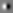
\includegraphics[width=0.2\columnwidth]{\figpath/filtering/Gx} &

\includegraphics[width=0.2\columnwidth]{\figpath/filtering/Gy} \\
(a) & (b)
\end{tabular}
%
\caption{First derivatives (a) $\Gx$ and (b) $\Gy = \Gx^T$}
\label{f:filters_firstderivs}
\end{figure}